\documentclass[../main-physics-problems.tex]{subfiles}
\begin{document}
\setcounter{section}{6}
\subsection{Free Fall Concepts}

\subsubsection{Gravitational Field Strength and Acceleration due to Gravity on Earth}



\begin{questions}

\question  
What is the value of the gravitational field strength on Earth's surface?  
\begin{randomizechoices}  
    \correctchoice \SI{10}{N/kg}  
    \choice \SI{1.0}{N/kg}  
    \choice \SI{8.9}{m/s^2}  
    \choice \SI{0}{m/s^2}  
\end{randomizechoices}  



\question  
How does the gravitational field strength on Earth relate to the acceleration due to gravity on Earth, assuming \( g = \SI{10}{m/s^2} \)?  

\begin{randomizechoices}  
    \correctchoice They are numerically equal but have different units.  
    \choice They are unrelated quantities.  
    \choice Gravitational field strength is larger.  
    \choice Acceleration due to gravity is larger.  
\end{randomizechoices}  



\question  
Which of the following correctly describes the unit of gravitational field strength?  

\begin{randomizechoices}  
    \correctchoice \SI{}{N/kg}  
    \choice \SI{}{m/s^2}  
    \choice \SI{}{kg \cdot m/s}  
    \choice \SI{}{N \cdot m^2/kg^2}  
\end{randomizechoices}  


\question 

A \SI{5}{kg} object is placed on Earth's surface. What is the magnitude of the gravitational force acting on the object?  
\begin{randomizechoices}  
    \correctchoice \SI{50}{N}  
    \choice \SI{5}{N}  
    \choice \SI{10}{N}  
    \choice \SI{100}{N}  
\end{randomizechoices}  



\question  
If the acceleration due to gravity on Earth were to decrease from \( g = \SI{10}{m/s^2} \), what would happen to the gravitational field strength?  

\begin{randomizechoices}  
    \correctchoice It would decrease.  
    \choice It would increase.  
    \choice It would stay the same.  
    \choice It would become negative.  
\end{randomizechoices}  
\end{questions}

\subsubsection{Why Objects near Earth's Surface Fall at the
Same Rate}

\begin{questions}  


\question  
Which of the following statements best explains why all objects near Earth’s surface fall at the same rate when in free fall?  

\begin{randomizechoices}  
    \correctchoice The gravitational force on an object is proportional to its mass, so the acceleration due to gravity is the same for all objects.  
    \choice Heavier objects experience more gravitational force, causing them to fall faster.  
    \choice Air resistance cancels out differences in mass, making objects fall at the same rate.  
    \choice The acceleration due to gravity decreases with altitude, which equalizes falling speeds.  
\end{randomizechoices}  


\question  
According to the law of universal gravitation, what determines the gravitational force acting on an object near Earth’s surface?  

\begin{randomizechoices}  
    \correctchoice The mass of the object, the mass of Earth, and the distance between the object and Earth’s center.  
    \choice Only the mass of the object and the distance from Earth’s surface.  
    \choice Only the mass of Earth and the object’s velocity.  
    \choice The object’s weight and its volume.  
\end{randomizechoices}  

\question  
How does Newton’s second law of motion (\( F_{\text{net}} = ma \)) help explain why objects in free fall have the same acceleration near Earth’s surface?  

\begin{randomizechoices}  
    \correctchoice The gravitational force (\( F_g = mg \)) is proportional to mass, so the mass cancels out when calculating acceleration, leaving \( g \) as the constant acceleration.  
    \choice The gravitational force depends on velocity, which ensures all objects accelerate equally.  
    \choice Air resistance balances the forces, resulting in equal acceleration.  
    \choice Gravitational force is independent of mass, so all objects fall at the same rate.  
\end{randomizechoices}  


\question  
What is the formula for the gravitational force acting on an object of mass \( m \) near Earth’s surface?  
\begin{randomizechoices}  
    \correctchoice \( F_g = mg \)  
    \choice \( F_g = \frac{Gm_1m_2}{r^2} \)  
    \choice \( F_g = \frac{1}{2}mv^2 \)  
    \choice \( F_g = m g^2 \)  
\end{randomizechoices}  



\question  
Why does the mass of an object not affect its acceleration in free fall?  
\begin{randomizechoices}  
    \correctchoice The gravitational force increases with mass, but the increased force is exactly offset by the increased inertia, resulting in the same acceleration.  
    \choice Gravitational force is independent of mass.  
    \choice Air resistance decreases with increased mass.  
    \choice Heavier objects have more inertia, so they fall slower.  
\end{randomizechoices}  

\end{questions}

\subsubsection{Final Velocity and Time in Free Fall}

\begin{questions}
\question
Which of the following factors does not affect the final velocity of an object in free fall?

\begin{randomizechoices}
\correctchoice Mass of the object
\choice Initial position of the object
\choice Initial velocity of the object
\choice Time the object has been falling
\end{randomizechoices}

\question
An object is dropped from rest at a height of 50 meters. If the object’s mass is doubled, how does its final velocity change just before it hits the ground?

\begin{randomizechoices}
\correctchoice The final velocity does not change.
\choice The final velocity is doubled.
\choice The final velocity is halved.
\choice The final velocity increases exponentially.
\end{randomizechoices}

\question
If an object is in free fall and has an initial velocity of \SI{0}{m/s}, how does the time it takes to reach the ground change if the object is dropped from a higher position?

\begin{randomizechoices}
\correctchoice The time increases.
\choice The time decreases.
\choice The time remains the same.
\choice The time becomes zero.
\end{randomizechoices}


\question
An object is thrown downward with an initial velocity. If the initial velocity is increased, what happens to the final velocity of the object just before hitting the ground?

\begin{randomizechoices}
\correctchoice The final velocity increases.
\choice The final velocity decreases.
\choice The final velocity stays the same.
\choice The final velocity becomes zero.
\end{randomizechoices}

\question
For an object in free fall after being thrown downward, which of the following will result in the shortest time for the object to reach the ground?

\begin{randomizechoices}
\correctchoice A higher initial velocity and a lower initial position.
\choice A lower initial velocity and a higher initial position.
\choice A higher initial position and zero initial velocity.
\choice A higher initial position and a lower initial velocity.
\end{randomizechoices}
\end{questions}

\clearpage

\subsubsection{Motion of Objects Dropped or Thrown using Multiple Representations}

\begin{questions}
\question  
An object is dropped from a height. Which of the following statements is true about its initial velocity?  

\begin{randomizechoices}  
    \correctchoice The initial velocity is zero.  
    \choice The initial velocity is equal to the velocity after 1 second.  
    \choice The initial velocity is constant and non-zero.  
    \choice The initial velocity is equal to the acceleration due to gravity.  
\end{randomizechoices}  

\question  
If an object is dropped from rest, what is its velocity after 3 seconds?  

\begin{randomizechoices}  
    \correctchoice \(\SI{30}{m/s}\)  
    \choice \(\SI{10}{m/s}\)  
    \choice \(\SI{15}{m/s}\)  
    \choice \(\SI{25}{m/s}\)  
\end{randomizechoices}  


\question  
An object is dropped from a height of 50 meters. How long does it take to reach the ground?  

\begin{randomizechoices}  
    \correctchoice 3.16 seconds  
    \choice 2.5 seconds  
    \choice 5.0 seconds  
    \choice 4.0 seconds  
\end{randomizechoices}  


\question  
What is the momentum of a 10 kg object that is moving downward with a velocity of \(\SI{20}{m/s}\)?  

\begin{randomizechoices}  
    \correctchoice \(\SI{200}{kg \cdot m/s}\)  
    \choice \(\SI{100}{kg \cdot m/s}\)  
    \choice \(\SI{50}{kg \cdot m/s}\)  
    \choice \(\SI{20}{kg \cdot m/s}\)  
\end{randomizechoices}  


\question  
An object is thrown upward with an initial velocity of \(\SI{20}{m/s}\). What is its velocity after 2 seconds of flight?  

\begin{randomizechoices}  
    \correctchoice \(\SI{0}{m/s}\)  
    \choice \(\SI{10}{m/s}\)  
    \choice \(\SI{-10}{m/s}\)  
    \choice \(\SI{-20}{m/s}\)  
\end{randomizechoices}  


\question  
An object is thrown upward with an initial velocity of \(\SI{15}{m/s}\). What is its maximum height?  

\begin{randomizechoices}  
    \correctchoice \(\SI{11.25}{m}\)  
    \choice \(\SI{7.5}{m}\)  
    \choice \(\SI{22.5}{m}\)  
    \choice \(\SI{15}{m}\)  
\end{randomizechoices}  


\question  
When an object is thrown downward with an initial velocity of \(\SI{5}{m/s}\), what is its velocity after 3 seconds?  

\begin{randomizechoices}  
    \correctchoice \(\SI{35}{m/s}\)  
    \choice \(\SI{30}{m/s}\)  
    \choice \(\SI{25}{m/s}\)  
    \choice \(\SI{40}{m/s}\)  
\end{randomizechoices}  


\question  
An object is dropped from a height of 20 meters. What is its kinetic energy just before hitting the ground? (Assume the mass of the object is 4 kg.)  

\begin{randomizechoices}  
    \correctchoice \(\SI{800}{J}\)  
    \choice \(\SI{400}{J}\)  
    \choice \(\SI{200}{J}\)  
    \choice \(\SI{1600}{J}\)  
\end{randomizechoices}  


\question  
What is the acceleration of an object in free fall that is dropped from rest?  

\begin{randomizechoices}  
    \correctchoice \(\SI{10}{m/s^2}\)  
    \choice \(\SI{0}{m/s^2}\)  
    \choice \(\SI{9.8}{m/s^2}\)  
    \choice \(\SI{20}{m/s^2}\)  
\end{randomizechoices}  


\question  
An object is thrown upward with an initial velocity of \(\SI{10}{m/s}\). What is the total time it will take for the object to return to its original position?  

\begin{randomizechoices}  
    \correctchoice 2 seconds  
    \choice 1 second  
    \choice 5 seconds  
    \choice 10 seconds  
\end{randomizechoices}  
\end{questions}

\clearpage

\subsubsection{Force, Impulse, and Work Done by Earth}

\begin{questions}
\question
.
\end{questions}

\subsection{Solving Constant Acceleration Problems}

\subsubsection{Describing What is Known About Motion}

\clearpage

\subsubsection{Solving for Unknown Quantities: Horizontal Motion}

\begin{questions}

\question
Coco the dog trots at \SI{2.0}{m/s}. When she hears her owner say ``Treat!'' she accelerates at \SI{1.2}{m/s^2} for \SI{4.0}{s}. What is Coco's final velocity?

\ifprintanswers
\bgroup
\color{red}
$v_f = v_i + at$
\egroup
\fi

\begin{choices}
    \choice \SI{4.8}{m/s}
    \correctchoice \SI{6.8}{m/s}
    \choice \SI{2.0}{m/s}
    \choice \SI{1.2}{m/s}
\end{choices}

\question 
Tom rides in a jet that accelerates from \SI{53.6}{m/s} to \SI{134}{m/s} at a rate of \SI{26.8}{m/s^2}. How long will it take Tom to reach his top velocity?

\ifprintanswers
\bgroup
\color{red}
$\displaystyle v_f = v_i + at \quad \Rightarrow \quad t = \frac{v_f - v_i}{a}$
\egroup
\fi

\begin{randomizechoices}
    \correctchoice \SI{3.0}{s}
    \choice \SI{4.0}{s}
    \choice \SI{9.0}{s}
    \choice \SI{16}{s}
\end{randomizechoices}


\question
Hurricane Iris crosses Cuba at \SI{5.0}{m/s}. When it reaches the ocean, it accelerates at \SI{0.48}{m/s^2} for \SI{35}{s}. What will be Hurricane Iris's final velocity?

\ifprintanswers
\bgroup
\color{red}
$v_f = v_i + at$
\egroup
\fi

\begin{randomizechoices}
    \correctchoice \SI{21.8}{m/s}
    \choice \SI{14.2}{m/s}
    \choice \SI{30.9}{m/s}
    \choice \SI{6.8}{m/s}
\end{randomizechoices}



\question
John is cruising in his car at \SI{35}{m/s} when the traffic light turns yellow, causing him to momentarily to hit the breaks. If he decelerates at \SI{-10}{m/s}, what will be his final velocity after \SI{3}{seconds}?

\ifprintanswers
\bgroup
\color{red}
$v_f = v_i + at$
\egroup
\fi

\begin{randomizechoices}
    \correctchoice \SI{5}{m/s}
    \choice \SI{10}{m/s}
    \choice \SI{65}{m/s}
    \choice \SI{25}{m/s}
\end{randomizechoices}

\question %43
A falcon moves in a straight line at a constant velocity of \SI{30}{m/s}. What is its displacement between $t = 0$ and $t = \SI{5.0}{s}$?

\begin{solution}
If the velocity is constant, the acceleration is zero: $a = 0$

\begin{align*}
    \Delta x &= v_i t + \frac{1}{2} a t^2 \\
    &= v_i t \\[1ex] 
    &= (\SI{30}{m/s})(\SI{5.0}{s}) \\[1ex]
    &= \boxed{\SI{150}{m}}
\end{align*}
\end{solution}

\question %44
Sonic, the hedgehog, starts at rest and moves in a straight line at a constant acceleration of \SI{30}{m/s^2}. What is Sonic's position at $t = \SI{5.00}{s}$ relative to his origin?

\begin{solution}
    \begin{align*}
        \Delta x &= v_i t +\frac{1}{2}a t^2 \\[1ex]
        &= (\SI{0}{m/s})(\SI{5.00}{s}) + \frac{1}{2}(\SI{30}{m/s^2})(\SI{5.00}{s})^2 \\[1ex]
        &= \boxed{\SI{375}{m}}
    \end{align*}
\end{solution}

\question %45
Now Sonic moves in a straight line with an initial velocity of \SI{30}{m/s} and constant acceleration \SI{30}{m/s^2}. 

\begin{parts}
\part What is his displacement at $t = \SI{5}{s}$?

\begin{solution}
\begin{align*}
    \Delta x &= v_i t +\frac{1}{2}a t^2 \\[1ex]
    &= (\SI{30}{m/s})(\SI{5.00}{s}) + \frac{1}{2}(\SI{30}{m/s^2})(\SI{5.00}{s})^2 \\[1ex]
    &= \boxed{\SI{525}{m}}
\end{align*}
\end{solution}

\part What is his velocity at this same time?

\begin{solution}
    \begin{align*}
        v_f &= v_i + at \\[1ex]
        &= \SI{30}{m/s} + (\SI{30}{m/s^2})(\SI{5.00}{s}) \\[1ex]
        &= \boxed{\SI{180}{m/s}}
    \end{align*}    
\end{solution}
\end{parts}

\question \label{openstax-2.20}
An Olympic-class sprinter starts a race with an acceleration of \SI{4.50}{m/s^2}. 

\begin{parts}
\part What is her speed \SI{2.40}{s} later?

\begin{solution}
\begin{align*}
    v_f &= v_i + at \\[1ex]
    &= \SI{0}{m/s} + (\SI{4.50}{m/s^2})(\SI{2.40}{s}) \\[1ex]
    &= \boxed{\SI{10.8}{m/s}}
\end{align*}
\end{solution}

\part Sketch a graph of her position vs. time for this period.
\begin{solution}
    \begin{center}
        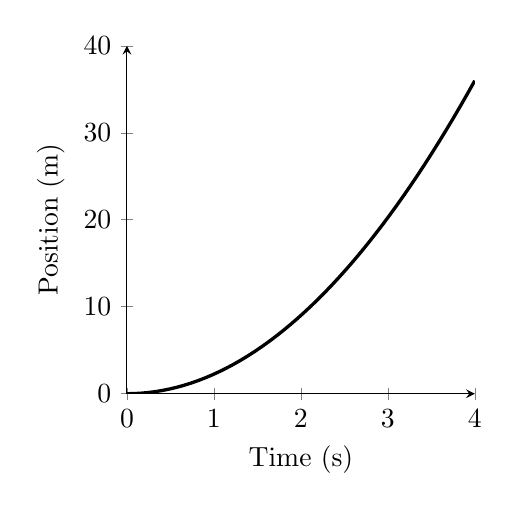
\begin{tikzpicture}
            \begin{axis}[
                width=6cm,height=6cm,
                axis lines=left,
                ylabel={Position (m)},
                xlabel={Time (s)},
                ymin=0,ymax=40,
                xmin=0,xmax=4,
            ]
            \draw[very thick] plot[domain=0:4,samples=50] (\x,{0.5*4.5*\x^2}); 
            \end{axis}
        \end{tikzpicture}
    \end{center}
\end{solution}
\end{parts}

\question \label{openstax-2.27}
In a slap shot, a hockey player accelerates the puck from a velocity of \SI{8.00}{m/s} to \SI{40.0}{m/s} in the same direction. If this shot takes \SI{3.33e-2}{s}, calculate the distance over which the puck accelerates.

\begin{solution}
\begin{align*}
    \Delta x &= \frac{1}{2} \left(v_i + v_f\right) t \\[1ex]
    &= \frac{1}{2} \left(\SI{8.00}{m/s} + \SI{40.0}{m/s}\right)(\SI{0.0333}{s}) \\[1ex]
    &= \boxed{\SI{0.799}{m}}
\end{align*}
\end{solution}

\question %53-ish
While entering a freeway, a car accelerates from rest at a rate of \SI{2.40}{m/s^2} for \SI{12.0}{s}. 

\begin{parts}
\part How far does the car travel in those \SI{12.0}{s}?

\begin{solution}
\begin{align*}
    \Delta x &= v_i t + \frac{1}{2} a t^2 \\[1ex]
    &= (\SI{0}{m/s})(\SI{12}{s}) + \frac{1}{2}(\SI{2.4}{m/s^2})(\SI{12.0}{s})^2 \\[1ex]
    &= \boxed{\SI{172.8}{m}}
\end{align*}
\end{solution}

\part What is the car's final velocity? 
\begin{solution}
\begin{align*}
    v_f &= v_i + a t \\[1ex]
    &=  \SI{0}{m/s} + (\SI{2.40}{m/s^2})(\SI{12.0}{s}) \\[1ex]
    &= \boxed{\SI{28.8}{m/s}}
\end{align*}
\end{solution}
\end{parts}

\begin{EnvUplevel}
    \textbf{Questions \ref{openstax-2.26}--\ref{kinematic-particle}}: K-level only.
\end{EnvUplevel}






\question \label{openstax-2.31}
A swan on a lake gets airborne by flapping its wings and running on top of the water. 

\begin{parts}
\part If the swan must reach a velocity of \SI{6.00}{m/s} to take off and it accelerates from rest at an average rate of \SI{0.350}{m/s^2}, how far will it travel before becoming airborne?

\begin{solution}
The swan's motion is govern by the equation

\begin{equation*}
    v_f^2 = v_i^2 + 2a \Delta x  
\end{equation*}

Solving for displacement leads to

\begin{align*}
    \Delta x &= \frac{v_f^2 - v_i^2}{2a} \\[1ex]
    &= \frac{(\SI{6.00}{m/s})^2 - (\SI{0}{m/s})^2}{2(\SI{0.350}{m/s^2})} \\[1ex]
    &= \boxed{\SI{51.4}{m}}
\end{align*}     
\end{solution}

\part How much time does it take the swan to become airborne?

\begin{solution}
The time interval for this acceleration is related by

\begin{equation*}
    v_f = v_i + at
\end{equation*}

Solving for time leads to

\begin{align*}
    t &= \frac{v_f - v_i}{a} \\[1ex]
    &= \frac{\SI{6.0}{m/s} - \SI{0}{m/s}}{\SI{0.350}{m/s^2}} \\[1ex]
    &= \boxed{\SI{17.1}{s}}
\end{align*}
\end{solution}
\end{parts}



\question %48
A particle has a constant acceleration of \SI{6.0}{m/s^2}. (a) If its initial velocity is \SI{2.0}{m/s}, at what time is its displacement \SI{5.0}{m}? (b) What is its velocity at that time?

\begin{solution}
    (a) We start with

    \begin{equation*}
        \Delta x = v_i t + \frac{1}{2} a t^2
    \end{equation*}

    and substitute the known values, leading to

    \begin{equation*}
        3 t^2 + 2 t - 5 = 0
    \end{equation*}

    which factors to

    \begin{equation*}
        (3t + 5)(t - 1) = 0
    \end{equation*}

    Taking the positive solution, we have
    
    \begin{equation*}
        \boxed{t = \SI{1.0}{s}}
    \end{equation*}
    
    (For a review on solving quadratic equations, see Example 7.74 of \href{https://openstax.org/books/elementary-algebra-2e/pages/7-6-quadratic-equations}{OpenStax: Elementary Algebra 2e}.)\medskip

    (b) The final velocity is

    \begin{align*}
        v_f &= v_i + a t \\[1ex] 
        &= \SI{2.0}{m/s} + (\SI{6.0}{m/s^2})(\SI{1.0}{s}) \\[1ex]
        &= \boxed{\SI{8.0}{m/s}}
    \end{align*}
\end{solution}

\question \label{openstax-2.26}
Blood is accelerated from rest to \SI{30.0}{cm/s} in a distance of \SI{1.80}{cm} by the left ventricle of the heart. How long does the acceleration take? Is the answer reasonable when compared with the time for a heartbeat?

\begin{solution}
Acceleration is related to initial and final velocities and displacement by

\begin{equation*}
    v_f^2 = v_i^2 + 2a \Delta x 
\end{equation*}

Solving for acceleration leads to

\begin{align*}
    a &= \frac{v_f^2 - v_i^2}{2 \Delta x} \\[1ex]
    &= \frac{(\SI{30}{cm/s})^2 - (\SI{0}{cm/s})^2}{2(\SI{1.80}{cm})} \\[1ex]
    &= \SI{250}{cm/s^2}
\end{align*}

The time interval for this acceleration is related by

\begin{equation*}
    v_f = v_i + at
\end{equation*}

Solving for time leads to

\begin{align*}
    t &= \frac{v_f - v_i}{a} \\[1ex]
    &= \frac{\SI{30}{cm/s} - \SI{0}{cm/s}}{\SI{250}{cm/s^2}} \\[1ex]
    &= \boxed{\SI{0.12}{s}}
\end{align*}
\end{solution}

\question \label{kinematic-particle} %49
At $t = \SI{10}{s}$, a particle is moving from left to right with a speed of \SI{5.0}{m/s}. At $t = \SI{20}{s}$, the particle is moving right to left with a speed of \SI{8.0}{m/s}. Assuming the particle's acceleration is constant, determine (a) its acceleration, (b) its initial velocity, and (c) the instant when its velocity is zero.

\begin{solution}
(a) The acceleration is

    \begin{equation*}
        a = \frac{v_2 - v_1}{t_2 - t_1} = \SI{-1.3}{m/s^2}
    \end{equation*}

(b) Starting with

    \begin{equation*}
        v_f = v_i + at
    \end{equation*}

    at $t = \SI{10}{s}$ and solving for initial velocity leads to

    \begin{align*}
        v_i &= v_f - at \\[1ex]
        &= \SI{5.0}{m/s} - (-\SI{1.3}{m/s^2}) (\SI{10}{s}) \\[1ex]
        &= \boxed{\SI{18}{m/s}}
    \end{align*}

    (c) Knowing initial velocity and acceleration from the previous parts, we set the final velocity equation to zero,

    \begin{equation*}
        v_f = v_i + a t = 0 \qquad ,
    \end{equation*}

    and solve for time:

    \begin{align*}
        t &= \frac{-v_i}{a} \\[1ex]
        &= \frac{-\SI{18}{m/s}}{\SI{-1.3}{m/s^2}} \\[1ex]
        &= \boxed{\SI{13.8}{s}}
    \end{align*}
\end{solution}


\end{questions}

\clearpage

\subsubsection{Solving for Unknown Quantities: Vertical Motion}

\begin{questions}

\question
A rock is dropped from rest from the top of a tall cliff, taking \SI{5.0}{s} to reach the ground. What is the magnitude of the acceleration due to gravity?

\begin{choices}
    \choice \SI{8.4}{m/s^2}
    \correctchoice \SI{10}{m/s^2}
    \choice \SI{4.9}{m/s^2}
    \choice \SI{245}{m/s^2}
\end{choices}


% \question \label{prob:cliff_rock1}
% What is the rock's acceleration after 10 seconds of motion? ($g = \SI{9.8}{m/s^2}$)

% \begin{choices}
% \choice $a = g$
% \choice $a < g$
% \correctchoice $a = -g$
% \choice $a > g$
% \end{choices}

\question \label{prob:cliff_rock2}
A person standing on the edge of a high cliff throws a rock straight up with an initial velocity of \SI{13.0}{m/s}. The rock misses the edge of the cliff as it falls back to earth. Calculate the position of the rock \SI{2.3}{s} after it is thrown.

\begin{choices}
    \correctchoice \SI{3.45}{m}
    \choice \SI{29.9}{m}
    \choice \SI{5.6}{m}
    \choice \SI{15.3}{m}
\end{choices}

\question \label{prob:cliff_rock3}
A person standing on the edge of a high cliff throws a rock straight up with an initial velocity of \SI{13.0}{m/s}. The rock misses the edge of the cliff as it falls back to earth. What is the velocity of the rock \SI{5.0}{s} after it is thrown?

\begin{choices}
    \correctchoice \SI{-37}{m/s}
    \choice \SI{-13}{m/s}
    \choice \SI{0}{m/s}
    \choice \SI{65}{m/s}
\end{choices}


\question
A \SI{3}{kg} rock is dropped from rest from a \SI{5}{m} tall cliff. What is the speed of the rock as it strikes the ground?

\begin{solution}
We start with 

\begin{equation*}
    v_f^2 = v_i^2 - 2g \Delta y
\end{equation*}

and take the square root of both sides:

\begin{align*}
    v_f &= \sqrt{v_i^2 - 2g \Delta y} \\[1ex]
    &= \sqrt{(\SI{0}{m/s})^2 - 2(\SI{10}{m/s^2})(-\SI{5}{m})} \\[1ex]
    &= \boxed{\SI{10}{m/s}}
\end{align*}
\end{solution}

\question
Now the \SI{3}{kg} rock is thrown upwards at \SI{20}{m/s} over the edge of a \SI{5}{m} tall cliff. What is the speed of the rock as it strikes the ground now?

\begin{solution}
We start with 

\begin{equation*}
    v_f^2 = v_i^2 - 2g \Delta y
\end{equation*}

and take the square root of both sides:

\begin{align*}
    v_f &= \sqrt{v_i^2 - 2g \Delta y} \\[1ex]
    &= \sqrt{(\SI{20}{m/s})^2 - 2(\SI{10}{m/s^2})(-\SI{5}{m})} \\[1ex]
    &= \boxed{\SI{22.4}{m/s}}
\end{align*}
\end{solution}


\end{questions}

\clearpage

\subsubsection{Multi-Step Problems with Kinematic Equations}

\begin{questions}
\question
In the procedure below, you will calculate your reaction time using only a ruler, a partner, and physics.

\begin{parts}
\part Measure the displacement of a ruler by taking the following steps:

\begin{minipage}{0.68\textwidth}
\centering
    \begin{enumerate}[itemsep=0pt,topsep=0pt]
        \item Partner 1 (P1) holds the ruler vertically, with centimeters increasing upwards.
        \item Partner 2 (P2) places the \SI{0.0}{cm} end between their index finger and thumb, leaving a small gap between the ruler and fingers.
        \item \label{step-drops} P1 unexpectedly drops the ruler from rest.
        \item P2 catches the ruler with two fingers as fast as possible. Their fingers will mark a location on the ruler between \SI{0}{cm} and \SI{30}{cm}. 
        \item \label{step-records} Using the table below, P2 records the location on the ruler where their fingers made the catch.
        \item Repeat steps \ref{step-drops}--\ref{step-records} three times.
        \item P2 calculates the average drop distance from the three values in their table.
        \item Partners 1 and 2 switch roles and repeat the steps above.
    \end{enumerate}
\end{minipage}%
\hspace{5mm}
\begin{minipage}{0.17\textwidth}
\centering
    \begin{tikzpicture}[scale=0.7]
        \clip (-2.2,5.5) -- (-2.2,-1.5) -- (1.5,-1.5) -- (1.5,5.5) -- cycle;
        \tkzRegle[Longueur=7,Rotation=90,Circles=false]
        \draw[ultra thick,<-,xshift=-2pt] (0,0) -- (-1.5,-0.8) node[below,align=center,xshift=5mm] {fingers here};
    \end{tikzpicture}
\end{minipage}

\end{parts}


\end{questions}
\clearpage

\begin{questions}





\question
If an object's acceleration is \SI{3}{m/s^2}, then with every second that passes, the object's velocity (speed) will increase by \fillin[][2cm]\ .

\begin{choices}
    \choice \SI{1}{m/s}
    \choice \SI{2}{m/s}
    \correctchoice \SI{3}{m/s}
    \choice \SI{4}{m/s}
\end{choices}



\question
What are the units used to measure acceleration?

\begin{choices}
    \choice meters per second (\SI{}{m/s})
    \correctchoice meters per second squared (\SI{}{m/s^2})
    \choice meters (m)
    \choice seconds (s)
\end{choices}


\question %This problem and the next one go together.
A subway train accelerates from rest to \SI{12.8}{m/s} (\SI{45.9}{km/h}) in \SI{17.0}{s}. What is the average acceleration during that time interval?

\begin{choices}
\choice \SI{12.8}{m/s}
\choice \SI{2.70}{m/s^2}
\choice \SI{45.9}{m/s^2}
\CorrectChoice \SI{0.753}{m/s^2} 
\end{choices}




\question
An object accelerates from \SI{120}{m/s} to \SI{145}{m/s} at a rate of \SI{7.5}{m/s^2}. How long will it take the object to reach its final velocity?

\begin{choices}
    \correctchoice \SI{3.3}{s}
    \choice \SI{4.9}{s}
    \choice \SI{0.3}{s}
    \choice \SI{25}{s}
\end{choices}


\question
The Houston Zoo releases a falcon from a cage. The falcon flies at \SI{5}{m/s}. When it sees its breakfast (a small mouse), it accelerates to \SI{32}{m/s} in \SI{7.2}{s}. What is the falcon's average acceleration?
%$a = \SI{3.75}{m/s^2}$



\question
What is acceleration?

\begin{choices}
\choice The rate of change of acceleration.
\choice The rate of change of position. 
\CorrectChoice The rate of change of velocity.
\choice The rate of change of time.
\end{choices}

\question %Like PCA
An elevator moves downward as its speed \textit{decreases}. What is the direction of its acceleration?

\begin{choices}
\choice Left
\choice Right 
\correctchoice Up
\choice Down
\end{choices}

\question %Like PCA
A car travels eastward as its speed \textit{increases}. What is the direction of its acceleration?

\begin{choices}
\choice North
\choice South 
\correctchoice East
\choice West
\end{choices}


\question % Like Ch2 #16
A cheetah can accelerate from rest to a speed of \SI{35.0}{m/s} in \SI{7.00}{s}. What is its acceleration?

\begin{choices}
\choice \SI{245}{m/s^2}
\choice \SI{0.309}{m/s^2}
\CorrectChoice \SI{5.00}{m/s^2}
\choice \SI{18.2}{m/s^2}
\end{choices}

\question % Like Ch2 #18
A commuter backs her car out of her garage with an acceleration of \SI{1.2}{m/s^2}. How long does it take her to reach a speed of \SI{2.4}{m/s}?

\begin{choices}
\choice \SI{2.9}{s}
\correctchoice \SI{2.0}{s}
\choice \SI{0.5}{s}
\choice \SI{3.6}{s}
\end{choices}


% \begin{choices}
% \choice \SI{6.9}{s}
% \choice \SI{1.5}{s}
% \CorrectChoice \SI{1.3}{s}
% \choice \SI{0.22}{s}
% \end{choices}

\question %Like OpenStax Physics Ch2 #8 https://openstax.org/books/physics/pages/3-critical-thinking-items

A motorcycle moving at a constant velocity suddenly accelerates at a rate of \SI{3.0}{m/s^2} to a speed of \SI{30}{m/s} in \SI{4.0}{s}. What was the initial speed of the motorcycle?

\begin{choices}
\choice \SI{0.0}{m/s}
\choice \SI{10}{m/s}
\choice \SI{12}{m/s}
\CorrectChoice \SI{18}{m/s}
\end{choices}

\question %Like Example 2.10 
Dragsters can achieve average accelerations of \SI{24.0}{m/s^2}. Suppose such a dragster accelerates from rest at this rate for \SI{4.00}{s}. How far does it travel in this time?

\begin{choices}
\choice \SI{48.0}{m}
\choice \SI{96.0}{m}
\correctchoice \SI{192}{m}
\choice \SI{6.00}{m}
\end{choices}

% \begin{solution}

% $a = \SI{24.0}{m/s^2}$, $v_0 = 0$, $t = \SI{4.00}{s}$. Let $x_0 = 0$

% $x =\ ?$

% \begin{equation*}
%     x = x_0 + v_0 t + \frac{1}{2} a t^2 = \SI{192}{m}
% \end{equation*}
% \end{solution}


%
\question %Like Ch2 #27
In a slap shot, a hockey player accelerates the puck from a velocity of \SI{5.0}{m/s} to \SI{85}{m/s} in the same direction. If this shot takes \SI{7.0e-2}{s}, calculate the distance over which the puck accelerates.

\begin{choices}
\choice \SI{0.35}{m}
\correctchoice \SI{2.8}{m}
\choice \SI{5.9}{m}
\choice \SI{5.6}{m}
\end{choices}

% \begin{solution}
% $v_0 = \SI{5.0}{m/s}$, $v = \SI{85}{m/s}$, $t = \SI{7.0e-2}{s}$. Let $x_0 = 0$.

% $x =\ ?$

% The average velocity is

% \begin{equation*}
%     \bar{v} = \frac{v_0 + v}{2} = \SI{40}{m/s}\ .
% \end{equation*}

% Therefore, distance traveled is

% \begin{equation*}
%     x = x_0 + \bar{v}t = \SI{2.8}{m}\ .
% \end{equation*}
% \end{solution}



\vspace{1em}
\hrule

\question %Like Ch2 #33
An unwary football player collides with a padded goalpost while running at a velocity of \SI{7.0}{m/s} and comes to a full stop after compressing the padding and his body \SI{0.50}{m}. What is his deceleration?

\begin{choices}
\choice \SI{-3.5}{m/s^2}
\choice \SI{-14}{m/s^2}
\correctchoice \SI{-49}{m/s^2}
\choice \SI{-9.8}{m/s^2}
\end{choices}

% \begin{solution}

% $v_0 = \SI{7.0}{m/s}$, $v = 0$, $\Delta{x} = x - x_0 = \SI{0.50}{m}$. 

% $a =\ ?$

% The known and unknown quantities are related by the kinematic equation

% \begin{equation*}
%     v^2 = v^2_0 + 2 a \left(x - x_0\right)
% \end{equation*}

% Solving for acceleration leads to

% \begin{equation*}
%     a = \frac{v^2 - v_0^2}{2 \left(x - x_0\right)} = \SI{-49}{m/s^2}\ .
% \end{equation*}
% \end{solution}










% 

\question
Which quantity is equal to the area under the curve of a \textbf{velocity vs.~time} graph?
\begin{choices}
\correctchoice displacement
\choice acceleration
\choice distance
\choice velocity
\end{choices}





\begin{EnvUplevel}
\textbf{The graph below represents a football player's motion, based on units of yards (yd). Refer to the graph for Questions \ref{prob:FootballPlayer1} through \ref{prob:FootballPlayer3}.}
\end{EnvUplevel}

\begin{figure}[h!]
    \centering
    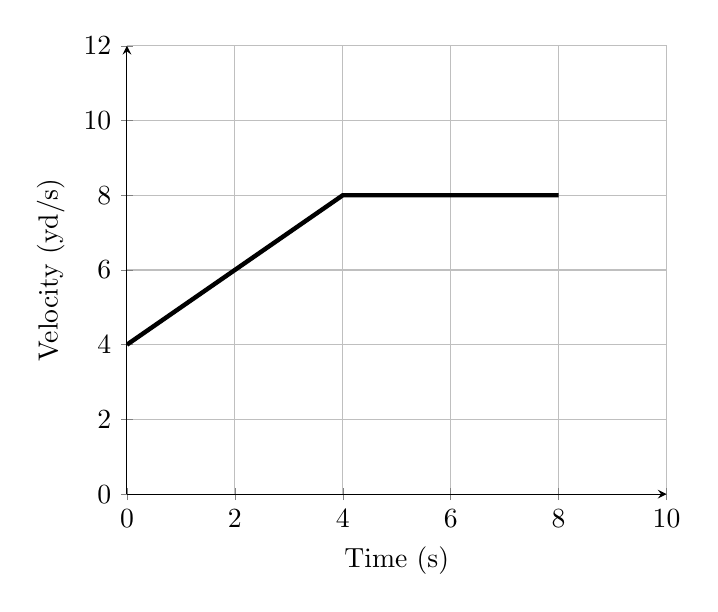
\begin{tikzpicture}
    \begin{axis}[axis y line=left, 
        axis x line=left,
        ymin=0, ymax=12,
        xmin=0, xmax=10,
        ylabel = Velocity (yd/s),
        xlabel = Time (s),
        grid=both,
        ytick={0,2,...,12}
    ]
    \addplot[
        %color=green!67!black,
        color=black,
        mark options={color=black},mark=none,
        ultra thick,
        ]
        coordinates {
        (0,4)
        (4,8)
        (8,8)
        };
    \end{axis}
    \end{tikzpicture}
    \label{fig:my_label}
\end{figure}

\question \label{prob:FootballPlayer1}
What is the player's \textbf{average acceleration} in the first 4 seconds?

\begin{choices}
\choice \SI{8}{yd/s^2}
\correctchoice \SI{1}{yd/s^2}
\choice \SI{4}{yd/s^2}
\choice \SI{2}{yd/s^2}
\end{choices}

\question \label{prob:FootballPlayer2}
What is the player's \textbf{average velocity} in the first 4 seconds?

\begin{choices}
\choice \SI{3}{yd/s}
\choice \SI{1}{yd/s}
\choice \SI{2}{yd/s}
\correctchoice \SI{6}{yd/s}
\end{choices}

\question \label{prob:FootballPlayer3}
If the player is at the 12-yard line at $t=0$, what is their \textbf{final position} at the end of the time interval?

\begin{choices}
\choice 64-yard line
\choice 8-yard line
\correctchoice 68-yard line
\choice 72-yard line
\end{choices}

\vspace{1em}
\hrule


\question
An object moves in accordance with the graph below. What is the object's acceleration?
\vspace{1em}

\begin{minipage}{0.3\textwidth}
    \begin{choices}
    \choice \SI{1}{m/s^2}
    \choice \SI{6}{m/s^2}
    \choice \SI{125}{m/s^2}
    \CorrectChoice \SI{5}{m/s^2}
    \end{choices}
\end{minipage}%
\begin{minipage}{0.3\textwidth}
\scalebox{0.8}{
    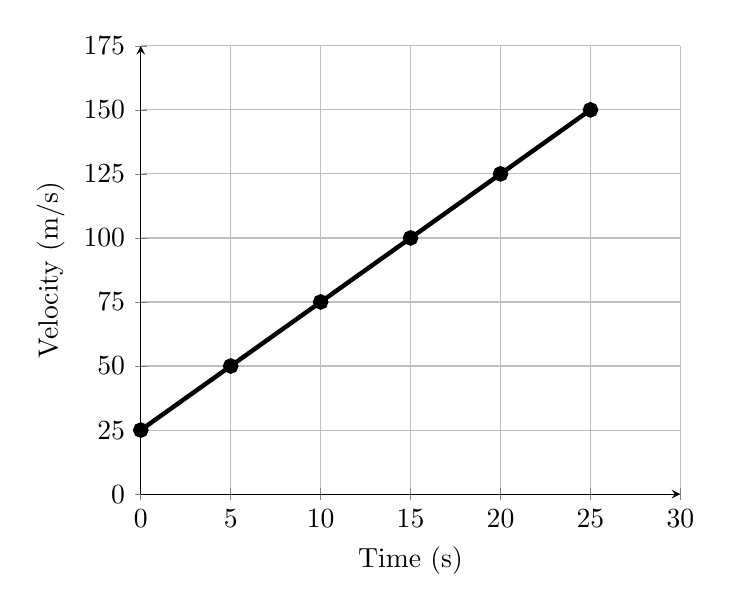
\begin{tikzpicture}
    \begin{axis}[axis y line=left, 
        axis x line=left,
        ymin=0, ymax=175,
        xmin=0, xmax=30,
        ylabel = Velocity (m/s),
        xlabel = Time (s),
        grid=both,
        ytick={0,25,...,175}
    ]
    \addplot[
        %color=green!67!black,
        color=black,
        mark options={color=black},mark=*,
        ultra thick,
        ]
        coordinates {
        (0,25)(5,50)(10,75)(15,100)(20,125)(25,150)
        };
    \end{axis}
    \end{tikzpicture}
    }
\end{minipage}







%%%%% END QUIZ 5 %%%%% END QUIZ 5 %%%%% END QUIZ 5 %%%%% END  QUIZ 5 %%%%% END QUIZ 5 %%%%%

%%%%% QUIZ 6 %%%%% QUIZ 6 %%%%% QUIZ 6 %%%%% QUIZ 6 %%%%% QUIZ 6 %%%%%


%
% \question %Like Example 2.10 
% Dragsters can achieve average accelerations of \SI{23.0}{m/s^2}. Suppose such a dragster accelerates from rest at this rate for \SI{4.45}{s}. How far does it travel in this time?

% \begin{solutionorbox}[2in]

% $a = \SI{23.0}{m/s^2}$, $v_0 = 0$, $t = \SI{4.45}{s}$. Let $x_0 = 0$

% $x =\ ?$

% \begin{equation*}
%     x = x_0 + v_0 t + \frac{1}{2} a t^2 = \SI{228}{m}
% \end{equation*}
% \end{solutionorbox}

% \question %Like Ch2 #20
% An Olympic-class sprinter starts a race with an acceleration of \SI{4.30}{m/s^2}. What is her speed \SI{2.10}{s} later?

% \begin{solutionorbox}[2in]

% $a = \SI{4.30}{m/s^2}$, $t = \SI{2.10}{s}$, $v_0 = 0$

% $v =\ ?$

% \begin{equation*}
%     v = v_0 + at = \SI{9.03}{m/s}
% \end{equation*}


% \end{solutionorbox}

% %
% \question %Like Ch2 #27
% In a slap shot, a hockey player accelerates the puck from a velocity of \SI{5.70}{m/s} to \SI{88.4}{m/s} in the same direction. If this shot takes \SI{7.73e-2}{s}, calculate the distance over which the puck accelerates.

% \begin{solutionorbox}[2in]
% $v_0 = \SI{5.70}{m/s}$, $v = \SI{88.4}{m/s}$, $t = \SI{7.73e-2}{s}$. Let $x_0 = 0$.

% $x =\ ?$

% The average velocity is

% \begin{equation*}
%     \bar{v} = \frac{v_0 + v}{2} = \SI{47.0}{m/s}\ .
% \end{equation*}

% Therefore, distance traveled is

% \begin{equation*}
%     x = x_0 + \bar{v}t = \SI{3.64}{m}\ .
% \end{equation*}
% \end{solutionorbox}

% \question %Like Ch2 #28
% A powerful motorcycle can accelerate from rest to \SI{31.2}{m/s} in only \SI{4.23}{s}. How far does it travel in that time?

% \begin{solutionorbox}[2in]

% $v_0 = 0$ (``from rest''), $v = \SI{31.2}{m/s}$, $t = \SI{4.23}{s}$. Let $x_0 = 0$.

% $x =\ ?$

% Average velocity is

% \begin{equation*}
%     \bar{v} = \frac{v_0 + v}{2} = \SI{15.6}{m/s}\ .
% \end{equation*}

% Therefore, distance traveled is

% \begin{equation*}
%     x = x_0 + \bar{v}t = \SI{66.0}{m}\ .
% \end{equation*}

% \end{solutionorbox}

% \question %Like Ch2 #33
% An unwary football player collides with a padded goalpost while running at a velocity of \SI{6.13}{m/s} and comes to a full stop after compressing the padding and his body \SI{0.411}{m}. What is his deceleration?

% \begin{solutionorbox}[2in]

% $v_0 = \SI{6.13}{m/s}$, $v = 0$, $\Delta{x} = x - x_0 = \SI{0.411}{m}$. 

% $a =\ ?$

% The known and unknown quantities are related by the kinematic equation

% \begin{equation*}
%     v^2 = v^2_0 + 2 a \left(x - x_0\right)
% \end{equation*}

% Solving for acceleration leads to

% \begin{equation*}
%     a = \frac{v^2 - v_0^2}{2 \left(x - x_0\right)} = \SI{-45.7}{m/s^2}\ .
% \end{equation*}
% \end{solutionorbox}




\begin{EnvUplevel}
\textbf{Refer to the graph below and answer the questions below.}

\begin{center}
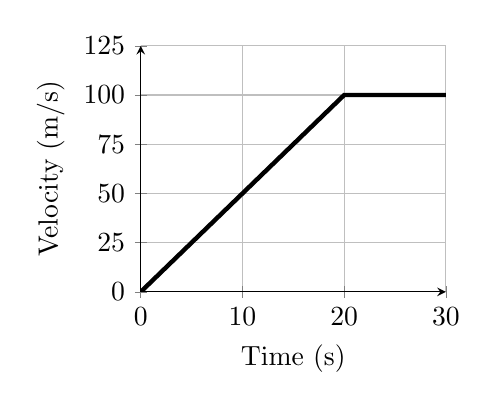
\begin{tikzpicture}
\begin{axis}[width=0.45\textwidth,
    axis y line=left, 
    axis x line=left,
    ymin=0, ymax=125,
    xmin=0, xmax=30,
    ylabel = Velocity (m/s),
    xlabel = Time (s),
    grid=both,
    ytick={0,25,...,175}
]
\addplot[
    %color=green!67!black,
    color=black,
    mark options={color=black},mark=none,
    ultra thick,
    ]
    coordinates {
    (0,0)(5,25)(10,50)(15,75)(20,100)(25,100)(30,100)
    };
\end{axis}
\end{tikzpicture}
\end{center}
\end{EnvUplevel}

\question
What is the \textbf{displacement} during the entire time interval?

\begin{solutionorbox}[2.5in]

For a \textbf{velocity vs.~time graph}, displacement is the area under the curve. 

\scalebox{0.8}{
\begin{tikzpicture}
\begin{axis}[color=black,axis y line=left, 
    axis x line=left,
    ymin=0, ymax=125,
    xmin=0, xmax=30,
    ylabel = Velocity (m/s),
    xlabel = Time (s),
    grid=both,
    ytick={0,25,...,175}
]

    \addplot[name path=f,domain=0:30,ultra thick,black] coordinates {(0,0)(20,100)(30,100)};

    \path[name path=axis] (axis cs:0,0) -- (axis cs:30,0);

    \addplot [
        thick,
        color=blue,
        fill=black!20!, 
        fill opacity=1
    ]
    fill between[
        of=f and axis,
        soft clip={domain=0:30},
    ];

\addplot[
    %color=green!67!black,
    color=black,
    mark options={color=black},mark=none,
    ultra thick,dashed,
    ]
    coordinates {
    (20,0)(20,100)
    };
\node at (axis cs:12,25) {\huge $A_1$};
\node at (axis cs:25,50) {\huge $A_2$};
\end{axis}
\end{tikzpicture}}

Dividing the graph at 20 seconds, the total area is composed of a right triangle of base \SI{20}{s} and height \SI{100}{m/s} ($A_1 = \frac{1}{2} \times \mathrm{base} \times \mathrm{height}$) and a rectangle of length \SI{10}{s} and width \SI{100}{m/s} ($A_2 = \mathrm{length} \times \mathrm{width}$).

Each area is

\begin{equation*}
    A_1 = \frac{1}{2}\left(\SI{20}{s}\right)\left(\SI{100}{m/s}\right) = \SI{1000}{m}
\end{equation*}

\begin{equation*}
    A_2 = (\SI{10}{s})(\SI{100}{m/s}) = \SI{1000}{m}
\end{equation*}

The total area, which equals the object's displacement, is

\begin{equation*}
    A = A_1 + A_2 = \SI{2000}{m}\ .
\end{equation*}

\end{solutionorbox}


\question
What is the \textbf{average velocity} during the first 20 seconds?

\begin{solutionorbox}[2.5in]

In the first 20 seconds, the corresponding initial and final velocities are $v_0 = 0$ and $v_f = \SI{100}{m/s}$. Average velocity under constant, non-zero acceleration is

\begin{equation*}
    \bar{v} = \frac{v_0 + v_f}{2} = \SI{50}{m/s}\ .
\end{equation*}

\end{solutionorbox}

\question %Like PCA
A skater starts at the top of a ramp and skates to the bottom. How is the skater's average acceleration calculated?

\begin{choices}
\CorrectChoice velocity at the \textbf{bottom} of the ramp \textit{minus} velocity at the \textbf{top}, \textit{divided} by the time it takes to reach the bottom
\choice velocity at the \textbf{top} of the ramp \textit{minus} velocity at the \textbf{bottom}, \textit{divided} by the time it takes to reach the bottom
\choice position at the \textbf{bottom} of the ramp \textit{minus} position at the \textbf{top}, \textit{divided} by the time it takes to reach the bottom
\choice position at the \textbf{top} of the ramp \textit{minus} position at the \textbf{bottom}, \textit{divided} by the time it takes to reach the bottom
\end{choices}


\question %Like PCA
An elevator moving down is slowing down. What is the direction of its acceleration?

\begin{choices}
\choice Left
\choice Right 
\correctchoice Up
\choice Down
\end{choices}

% \question %Like PCA
% A car moving to the right is speeding up. What is the direction of its acceleration?

% \question %Like PCA
% A car moving to the left is slowing down. What is the direction of its acceleration?

% \question %Like PCA
% A car moving to the left is speeding up. What is the direction of its acceleration?

% \question %Like PCA
% An elevator moving downward is slowing down. What is the direction of its acceleration?

% \question %Like PCA
% An elevator moving downward is speeding up. What is the direction of its acceleration?

% \begin{choices}
% \choice Up
% \choice Right
% \choice Left
% \CorrectChoice Down
% \end{choices}

% \question %Like PCA
% An elevator moving upward is slowing down. What is the direction of its acceleration?

% \question
% An elevator moving upward is speeding up. What is the direction of its acceleration?




\question % Like Ch2 #12
The driver of a sports car traveling at \SI{12.5}{m/s} steps down hard on the accelerator for \SI{4.5}{s} and the velocity increases to \SI{57.0}{m/s}. What was the average acceleration of the car during the \SI{4.5}{s} time interval?

\begin{choices}
\choice \SI{12.6}{m/s^2}
\choice \SI{2.7}{m/s^2}
\CorrectChoice \SI{9.9}{m/s^2}
\choice \SI{0.10}{m/s^2}
\end{choices}

\question % Like Ch2 #18
If a velocity increases from 0 to 36 m/s in 12 s, what is the average acceleration?

\begin{choices}
\choice \SI{0.333}{m/s^2}
\CorrectChoice \SI{3.0}{m/s^2}
\choice \SI{36}{m/s^2}
\choice \SI{432}{m/s^2}
\end{choices}

\question
What is average acceleration?

\begin{choices}
    \choice change in velocity divided by change in position
    \correctchoice change in velocity divided by change in time
    \choice rate of change of displacement
    \choice rate of change of position
\end{choices}

\question
Acceleration may be measured in units of \fillin\ .

\begin{choices}
    \choice meters per second (\SI{}{m/s})
    \correctchoice meters per second squared (\SI{}{m/s^2})
    \choice meters squared per second (\SI{}{m^2/s})
    \choice seconds (s)
\end{choices}

\question
If a falcon is flying at \SI{10}{m/s} and then, some short time later, flies at \SI{17}{m/s}, what is the falcon's change in velocity?

\begin{choices}
    \choice It's not possible to know without knowing the change in time.
    \choice \SI{10}{m/s}
    \choice \SI{17}{m/s}
    \correctchoice \SI{7.0}{m/s}
\end{choices}

\question
Amanda jogs with a constant velocity of \SI{6.2}{m/s} for 3.0 seconds. What is her average acceleration?

\begin{choices}
    \choice \SI{2.06}{m/s^2}
    \choice \SI{0.48}{m/s^2}
    \choice \SI{6.2}{m/s^2}
    \correctchoice \SI{0.0}{m/s^2}
\end{choices}

\question % Like Ch2 #18
The velocity of an airplane increases from 0 to \SI{36}{m/s} in \SI{12}{s}. What is the plane's average acceleration?

\begin{choices}
\choice \SI{0.333}{m/s^2}
\CorrectChoice \SI{3.0}{m/s^2}
\choice \SI{36}{m/s^2}
\choice \SI{432}{m/s^2}
\end{choices}

\question
An object moves in accordance with the graph below. What is the object's acceleration?
\vspace{1em}

\begin{minipage}{0.3\textwidth}
    \begin{choices}
    \choice \SI{1}{m/s^2}
    \choice \SI{6}{m/s^2}
    \choice \SI{125}{m/s^2}
    \CorrectChoice \SI{5}{m/s^2}
    \end{choices}
\end{minipage}%
\begin{minipage}{0.3\textwidth}
    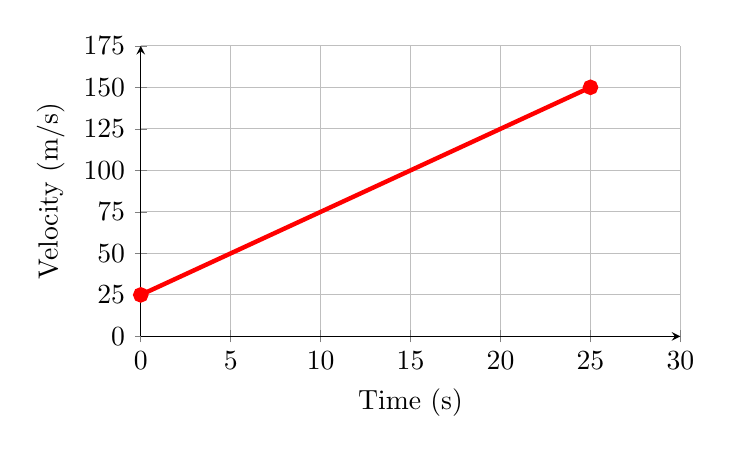
\begin{tikzpicture}
    \begin{axis}[width=240pt, height=150pt,
    axis y line=left, 
        axis x line=left,
        ymin=0, ymax=175,
        xmin=0, xmax=30,
        ylabel = Velocity (m/s),
        xlabel = Time (s),
        grid=both,
        ytick={0,25,...,175}
    ]
    \addplot[
        %color=green!67!black,
        color=red,
        mark options={color=red},mark=*,
        ultra thick,
        ]
        coordinates {
        (0,25)(25,150)
        };
    \end{axis}
    \end{tikzpicture}
\end{minipage}




\question
What is the acceleration of an object whose motion is shown by the graph below?

\begin{minipage}{0.3\textwidth}
    \begin{choices}
        \choice \SI{-52.5}{m/s^2}
        \choice \SI{3}{m/s^2}
        \choice \SI{52.5}{m/s^2}
        \correctchoice \SI{-3}{m/s^2}
    \end{choices}
\end{minipage}%
\begin{minipage}{0.3\textwidth}
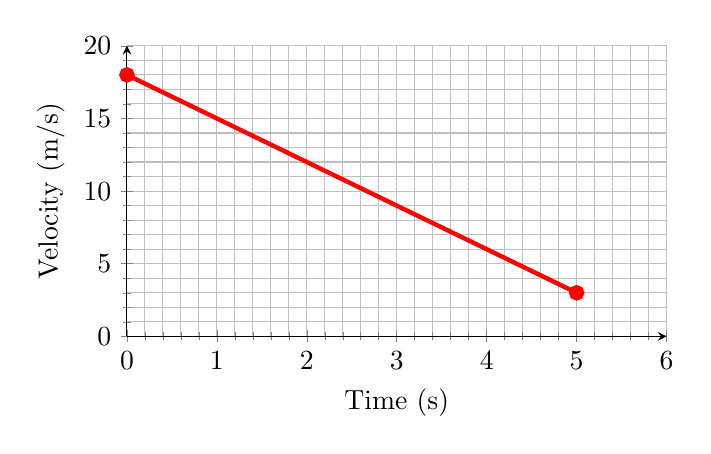
\begin{tikzpicture}
\begin{axis}[width=240pt, height=150pt,
        axis y line=left, 
        axis x line=left,
        ymin=0, ymax=20,
        xmin=0, xmax=6,
        ylabel = Velocity (m/s),
        xlabel = Time (s),
        grid=both,
        ytick={0,5,...,20},
        yminorgrids=true, minor y tick num=4,
        xminorgrids=true, minor x tick num=4,
    ]
    \addplot[
        color=red,
        mark options={color=red},mark=*,
        ultra thick,
        ]
        coordinates {
        (0,18)(5,3)
        };
\end{axis}
\end{tikzpicture} 
\end{minipage}

\question
Mario the soccer player jogs in one direction at a constant velocity in accordance with the graph below. What is his displacement?

\begin{minipage}{0.3\textwidth}
    \begin{choices}
        \choice \SI{0.0}{m}
        \correctchoice \SI{56}{m}
        \choice \SI{7}{m}
        \choice \SI{15}{m}
    \end{choices}
\end{minipage}%
\begin{minipage}{0.3\textwidth}
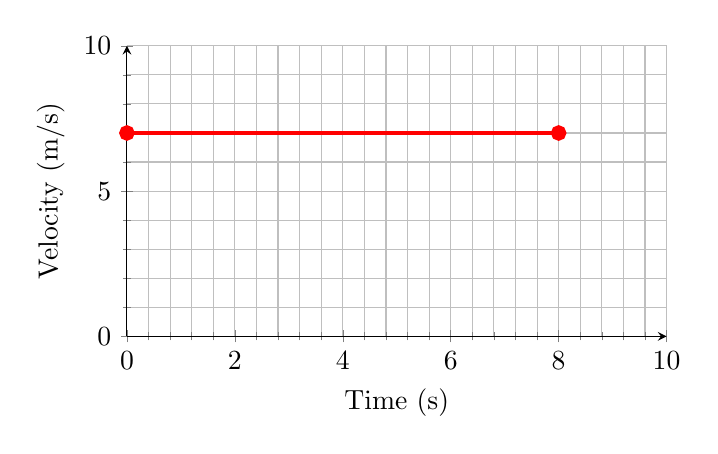
\begin{tikzpicture}
\begin{axis}[width=240pt, height=150pt,
        axis y line=left, 
        axis x line=left,
        ymin=0, ymax=10,
        xmin=0, xmax=10,
        ylabel = Velocity (m/s),
        xlabel = Time (s),
        grid=both,
        ytick={0,5,...,10},
        % ymajorgrids=true,
        % xmajorgrids=true,
        yminorgrids=true, minor y tick num=4,
        xminorgrids=true, minor x tick num=4,
    ]
    %\fill[black!20] (axis cs: 0,0) rectangle (axis cs: 6,15);
    \addplot[
        color=red,
        mark options={color=red},mark=*,
        ultra thick,
        ]
        coordinates {
        (0,7)(8,7)
        };
\end{axis}
\end{tikzpicture}
\end{minipage}

\question
An object's motion is represent by the graph below. What is the object's displacement?

\begin{minipage}{0.3\textwidth}
    \begin{choices}
        \correctchoice \SI{-15}{m}
        \choice \SI{15}{m}
        \choice \SI{-105}{m}
        \choice \SI{105}{m}
    \end{choices}
\end{minipage}%
\begin{minipage}{0.3\textwidth}
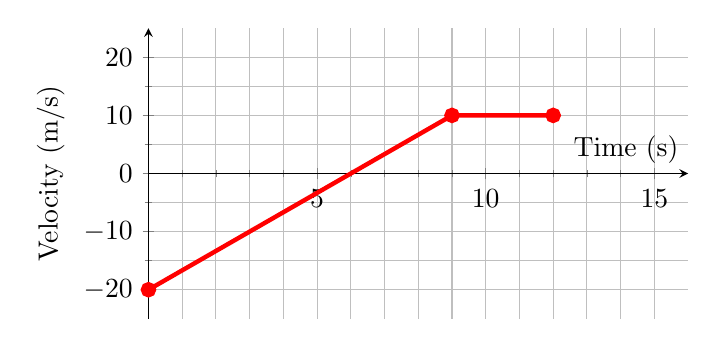
\begin{tikzpicture}
\begin{axis}[width=240pt,height=150pt,
    axis y line=left, 
    axis x line=center,
    xlabel = Time (s),
    ylabel = Velocity (m/s),
    ymin=-25, ymax=25,
    xmin=0, xmax=16,
    ytick={-20,-10,...,20},
    xtick={0,5,...,15},
    ymajorgrids=true,
    xmajorgrids=true,
    yminorgrids=true, minor y tick num=1,
    xminorgrids=true, minor x tick num=4,
    % x label style={anchor=west},
    clip=false,
]
    \addplot[
        %color=green!67!black,
        color=red,
        mark options={color=red},mark=*,
        ultra thick,
        ]
        coordinates {
        (0,-20)
        (9,10)
        (12,10)
        };
\end{axis}
\end{tikzpicture}
\end{minipage}

\end{questions}
\end{document}